\documentclass{amsart}

\usepackage{fullpage,amsmath,amssymb,graphicx}
\usepackage[caption=true]{subfig}
\usepackage{caption}
% \usepackage{caption,subcaption}
\usepackage{hyperref}
\captionsetup[subfigure]{margin=0pt, parskip=0pt, hangindent=0pt, indention=0pt, 
    labelformat=parens, labelfont=rm}


\DeclareMathOperator{\sgn}{sgn}

\begin{document}

\title{Notes for implementation  of Vitaly-Anatoly's scheme on a network}

\author{Shriram Srinivasan}
\address{LANL}
\email{shrirams@lanl.gov}



%%
%%  LaTeX will not make the title for the paper unless told to do so.
%%  This is done by uncommenting the following.
%%

\maketitle

\section{Introduction}

For a single pipe, the scheme is easy to understand and implement when given the initial conditions and the boundary conditions. However,  complications arise when we apply it for a network of pipes and compressors.

To start with, for each pipe, assume a base grid  of  pressure/density $(p/\rho)$ that matches the end-points, so that the grid for flux $\phi$ is staggered.  

Given initial conditions for both variables (pressure/density at $t_0$ and flux at $t_0 + \Delta t/2$), it is possible to advance all the internal nodes for density to the next time instant ($t_0 + \Delta t$) by using the discretized equation of balance of mass.  The pressure at the junctions however, cannot be calculated independently, and we need to satisfy the nodal balance to get the junction pressures for $t_0 + \Delta t$.

For this we shall use the flux at the end points, corresponding to the values at the ghost points, given by
\begin{align}
 s \phi_R^{n+1/2} = -\frac{s \Delta x}{\Delta t}\rho^{n+1} + \frac{s \Delta x}{\Delta t}\rho^{n} + s\phi_R^{-} \\
 s \phi_L^{n+1/2} = \frac{s \Delta x}{\Delta t}\rho^{n+1} - \frac{s \Delta x}{\Delta t}\rho^{n} + s\phi_L^{-}
\end{align}
where $\phi_R^{-}, \phi_L^{-1}$ are the internal nodes for flux closest to the ghost points. 
We use the letters $L, R$ to denote the left and right ends, where flow is assumed to be from left to right.
Substituting these equations into a nodal balance for the fluxes converts them into equations for junction pressure which can then be solved for.

\section{Junction without compressors}

At a node, say $i_0$, suppose there are incoming pipes $i_1, i_2, i_3, \dotsc$, outgoing pipes $o_1, o_2, o_3, ...$, and supply $q_{i_0}(t)$. We assume that for pipe $i$, $\sgn(i) = +1$ if incoming, and $-1$ if outgoing, and supply is positive, withdrawal is negative. The notation $u \in e(i_0)$ will be used to denote a pipe $u$ that has node $i_0$ as one end. 

Then, we can substitute pipe fluxes in terms of densities from above to get
\begin{equation}
\left[\sum_{u \in e(i_0)}\frac{s_u \Delta x_u}{\Delta t}\right]\rho^{n+1}(i_0) = q_{i_0}(t) + \left[\sum_{u \in e(i_0)}\frac{s_u \Delta x_u}{\Delta t}\right]\rho^{n}(i_0) + \sum_{u \in e(i_0)}\sgn(u) s_u \phi_{u}^-(i_0) 
\end{equation}
where $\phi_{u}^-(i_0)$ indicates that we want the flux value $\phi^-$ at the end $i_0$ for the pipe $u$, and $s_u$ stands for cross-sectional area of pipe $u$.

This equation can be solved for $\rho^{n+1}(i_0)$ since everything else is known.

Thus the algorithm may be understood as the sequence of steps:
\begin{enumerate}
\item Given $\rho^n$ everywhere, and $\phi^{n+1/2}$ at all internal nodes in network (initial condition)	
 \item Calculate $\rho^{n+1}$ for all internal nodes of all pipes 
 \item Find $\rho^{n+1}$ on pipe boundary (graph nodes)
 \item Now calculate $\phi^{n+1 + 1/2}$ for all \emph{internal} nodes of all pipes
 \item $phi^{n+1/2}$ at pipe ends can only be calculated when $\rho^n, \rho^{n+1}$ are known.
 \end{enumerate} 
Note that if the node $i_0$ is a \emph{slack node}, then the pressure $p(i_0)$ is always known and there is nothing to do.


\section{Junction with compressors}
For a compressor $c$ between nodes $i$ and $j$, it is assumed that the flow is unidirectional only. That is, \emph{we do not deal with flows wherein $\alpha \geq 1$ in one flow direction and $\alpha=1$  if  flow is in the reverse direction.} 
Moreover, one of the following \emph{must} be known/given: \\
(a) mass flow through compressor $f_c(t)$ \\
(b) Compressor ratio $\alpha_c(t)$ \\
(c) Discharge pressure of compressor \\ 

\subsection{Mass flow given}

If at a node $i_0$, we have a compressor with condition (a), we can treat the given mass flux $f_c(t)$ as a supply term and add $\sgn(c)f_c(t)$ on the RHS. Once again, the sign is +1 for incoming compressor and -1 for outgoing.
Same process is followed if we have multiple compressors at a node $i_0$ with condition (a).

\subsection{Compressor ratios given}

For reasons that will become clear subsequently, we assume that our network is such that if a compressor $c$ has nodes $i$ and $j$, at least one of $i$ or $j$  must be such that $c$ is the only compressor attached to that node. Let us record the implication of this statement  carefully.
This statement \emph{does not} rule out nodes where multiple compressors connect. Neither does it prohibit  such nodes from being neighbours. It only prevents the connecting edge between two such nodes from being a compressor. Stated another way, if nodes $i, j$ have multiple compressors, our assumption rules out a compressor connecting $i,j$, but a pipe may still connect $i, j$. 

Given a network satisfying the restriction, let us start by considering all \emph{slack} nodes first.
At a slack node $i_0$, if there is a compressor $c$ with compressor ratio $\alpha_c$, then the density at the node lying at other end of  the compressor is given by multiplying factor $\alpha_c$ if compressor is outgoing at $i_0 \; (\sgn(c) = -1$, but the factor is $1/\alpha_c$ when $\sgn(c) = +1$, i.e., incoming at $i_0$.



Now for a non-slack node $i_0$, we have multiple incoming/outgoing, incoming compressor $ic$ and outgoing compressor $oc$ whose ends are nodes $I$ and $O$ respectively.
Let us suppose that at the other end of $ic$, which is node $I$, there is supply $q_{I}(t)$, and pipes $e(I)$ and similarly for compressor $oc$ at node $O$.

Then, we have $\rho^{n+1}(i_0) = N/D$ 
where
\begin{align*}
N = & \sum_{u \in e(i_0)}\frac{s_u \Delta x_u}{\Delta t}\rho^n(i_0) +  \sum_{u \in e(i_0) }\sgn(u) s_u \phi_{u}^-(i_0) + q_{i_0}(t) \\ 
& \sum_{v \in e(I)}\frac{1}{\alpha_{ic}} \frac{s_{v} \Delta x_{v}}{\Delta t} \rho^n(i_0) + 
+ \sum_{v \in e(I)}\sgn(v) s_{v} \phi_{v}^-(I) + q_I(t) \\
& \sum_{w \in e(O)}\alpha_{oc} \frac{s_{w} \Delta x_{w}}{\Delta t} \rho^n(i_0) 
\sum_{w \in e(O)}\sgn(w) s_{w} \phi_{w}^-(O) +  q_{O}(t)   \\
\end{align*}


and $$D = \sum_{u \in e(i_0)}\frac{s_u \Delta x_u}{\Delta t} + 
\sum_{v \in e(I)}\frac{1}{\alpha_{ic}} \frac{s_{v} \Delta x_{v}}{\Delta t}  + 
\sum_{w \in e(O)}\alpha_{oc} \frac{s_{w} \Delta x_{w}}{\Delta t} $$

We can now see that the assumption we made about the network prevents the stencil for the given node from expanding further than  the other end of the compressors.

\subsection{Delivery pressure given}

If at node $i_0$, there are multiple pipes but  a single compressor $c$ (from node $I$) that delivers with given pressure $p(i_0)$, then one can write
\begin{equation}
\sum_{u \in e(i_0)} \sgn(u) s_u\phi_u^{n+1/2}(i_0) + f_c(t) = q_{i_0}(t) 
\end{equation}
Now $\phi_u(i_0)$ may be computed in terms of $\rho^{n+1}(i_0), \rho^{n}(i_0), \phi_{u}^-(i_0)$ so that one solves for $f_c(t)$. Once known, the flux is used at node $I$ on other end of $c$ to find the pressure, and thus the value of $\alpha$ is determined.

Let us write out the final equation after eliminating $f_c(t)$.

\begin{align*}
D = & \sum_{v \in e(I)} \frac{s_{v} \Delta x_{v}}{\Delta t} \\
N = & \left[\sum_{v \in e(I)} \frac{s_{v} \Delta x_{v}}{\Delta t}\right]\rho^n(I) + 
\sum_{v \in e(I)}\sgn(v) s_{v} \phi_{v}^-(I) + q_{I}(t) \\
& + \left[\sum_{u \in e(i_0)} \frac{s_{u} \Delta x_{u}}{\Delta t}\right][\rho^n(i_0) - \rho^{n+1}(i_0)] + \sum_{u \in e(i_0)}\sgn(u) s_{u} \phi_{u}^-(i_0) + q_{i_0}(t) \\
\rho^{n+1}(I) = & N/D \\
\end{align*}


Note that if there are two compressors delivering to same node with a given delivery pressure, then it is not possible to  solve for both mass flows from one equation. Even if we develop equations for the nodes at other end of the compressors, $\alpha$ being unknown means that we cannot eliminate any quantities and solve. This is a limitation of this formulation and hence 
\emph{we shall not consider networks where, at a node more than one compressor delivers with specified pressure.}

\subsection{Combination of above given}
Let us introduce the terms Level 0 and Level 1 vertices to formalize the network restrictions alluded to in the previous section. At a Level 0 vertex there are no incoming or outgoing compressors. At a Level 1 vertex, there can be compressors attached, but the vertex at the other end of each compressor has \emph{no other} compressors incoming or outgoing. If this is not true, then it is a Level 2 vertex.
Thus, for compressors attached at a Level 1 vertex, the other ends are all Level 2 vertices. 

The idea behind the classification is that to solve for pressure/density at a Level 0 vertex, information at that particular vertex alone is sufficient. At a Level 1 vertex, on the other hand, one needs information at that vertex, and information at the vertices that are the ends of the compressors incoming/outgoing. 


\begin{figure}[htb]
\centering
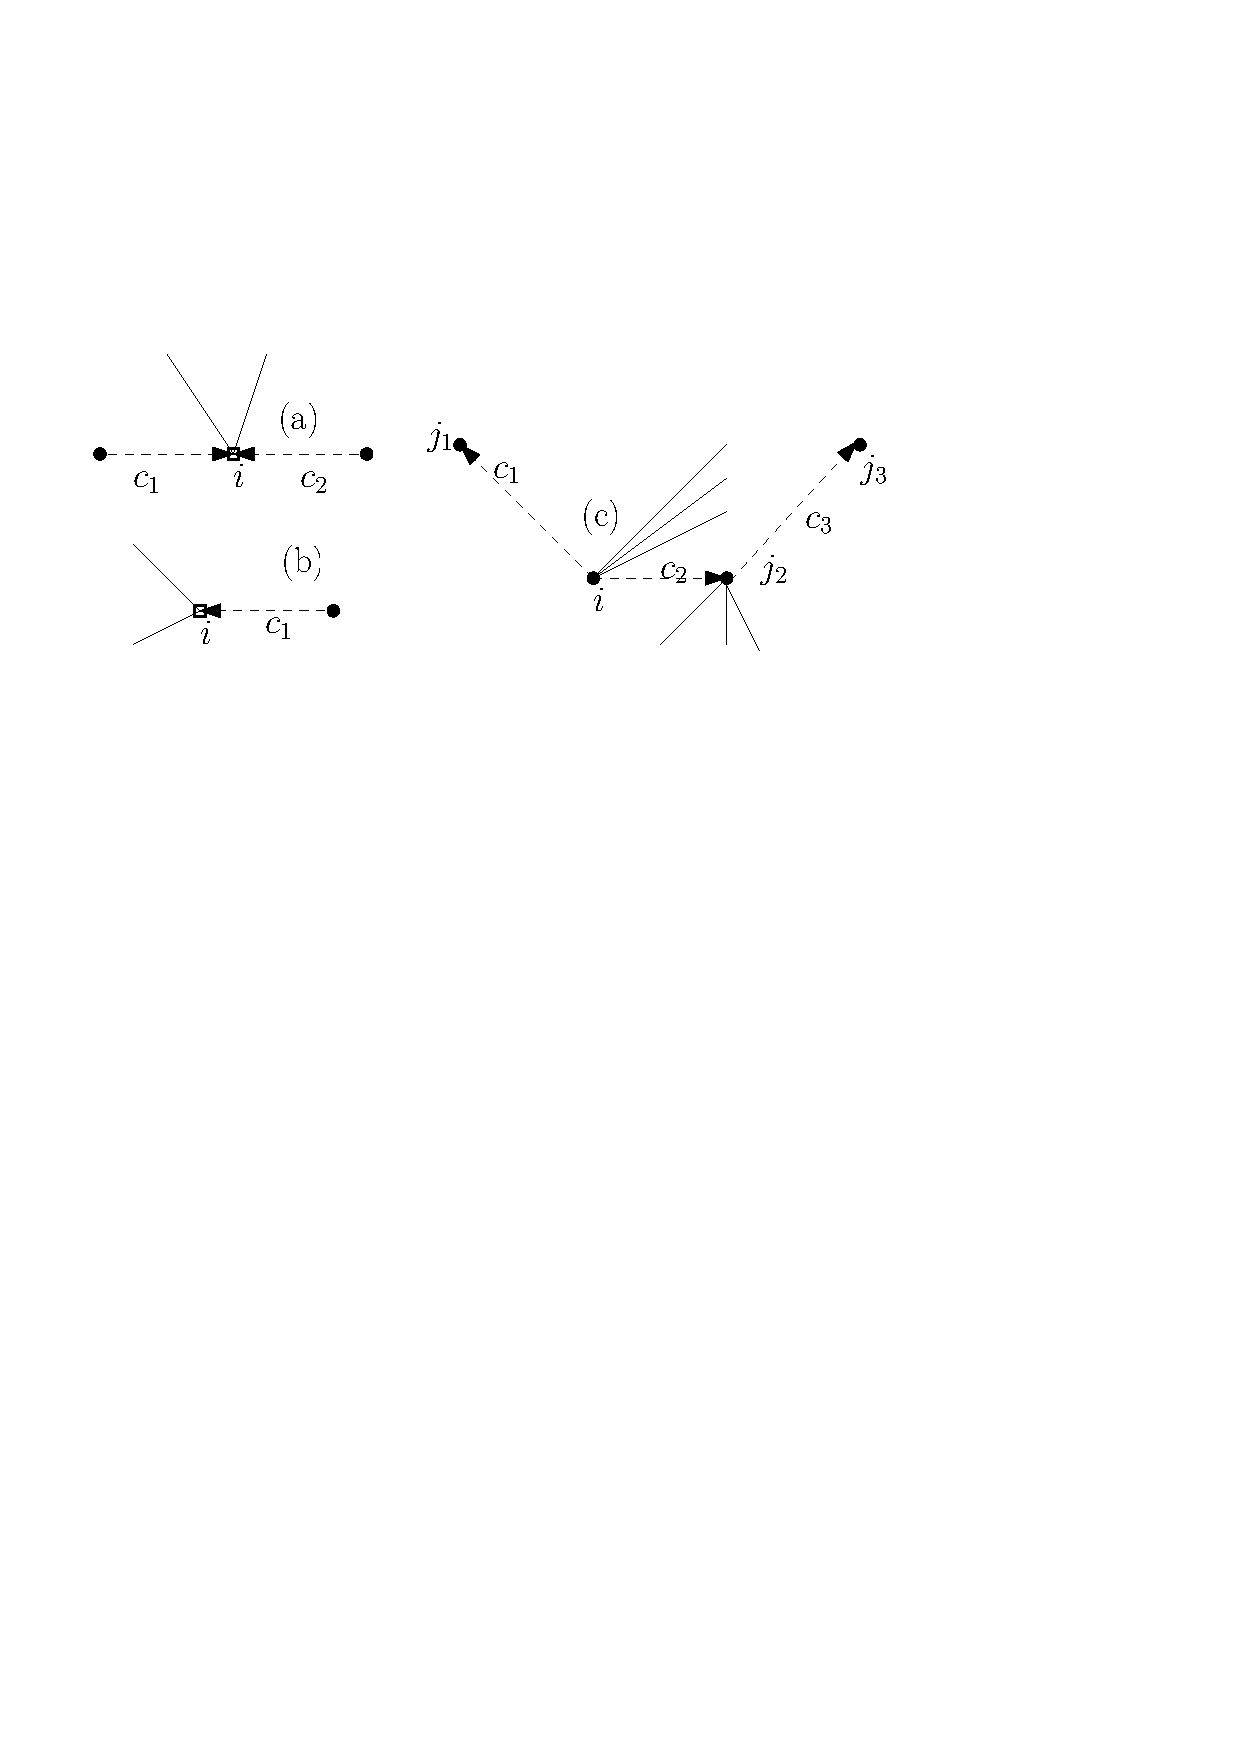
\includegraphics[scale=1]{pathologies}
\caption{Illustration of the three topologies that are explicitly forbidden. (a) Two incoming compressors at $i$ with discharge pressure control, (b) a slack node $i$ with incoming compressor that has discharge pressure control, and (c) connected Level 2 nodes due to three compressors in series.}
\label{fig:pathologies}
\end{figure}

We shall assume that the network satisfies three conditions: \\
(1) Two Level 2 vertices cannot be neighbours, i.e., Level 2 vertices can only have Level 1 neighbours. This condition can be stated  alternatively as: there can be at most two compressor elements in series in the network \\
(2) A vertex cannot be the delivery end of two  compressors with delivery pressure controls \\
(3) A vertex cannot be a  slack node and the delivery end of a  compressor simultaneously \\
These conditions are not very restrictive in reality and are simply pathological cases we want to avoid (See Figure~\ref{fig:pathologies}).
For networks that satisfy the above restrictions, we shall write down the equations for the pressure of a  general Level 1 vertex (and its Level 2 neighbours) in two common configurations (Figure~\ref{fig:configs}). Thus, if we can cycle through all Level 1 vertices of the network and calculate the densities, then all Level 2 neighbour vertices can be updated automatically, ensuring all vertices do get updated.



\begin{figure}[htb]
\centering
\subfloat[Configuration 1]{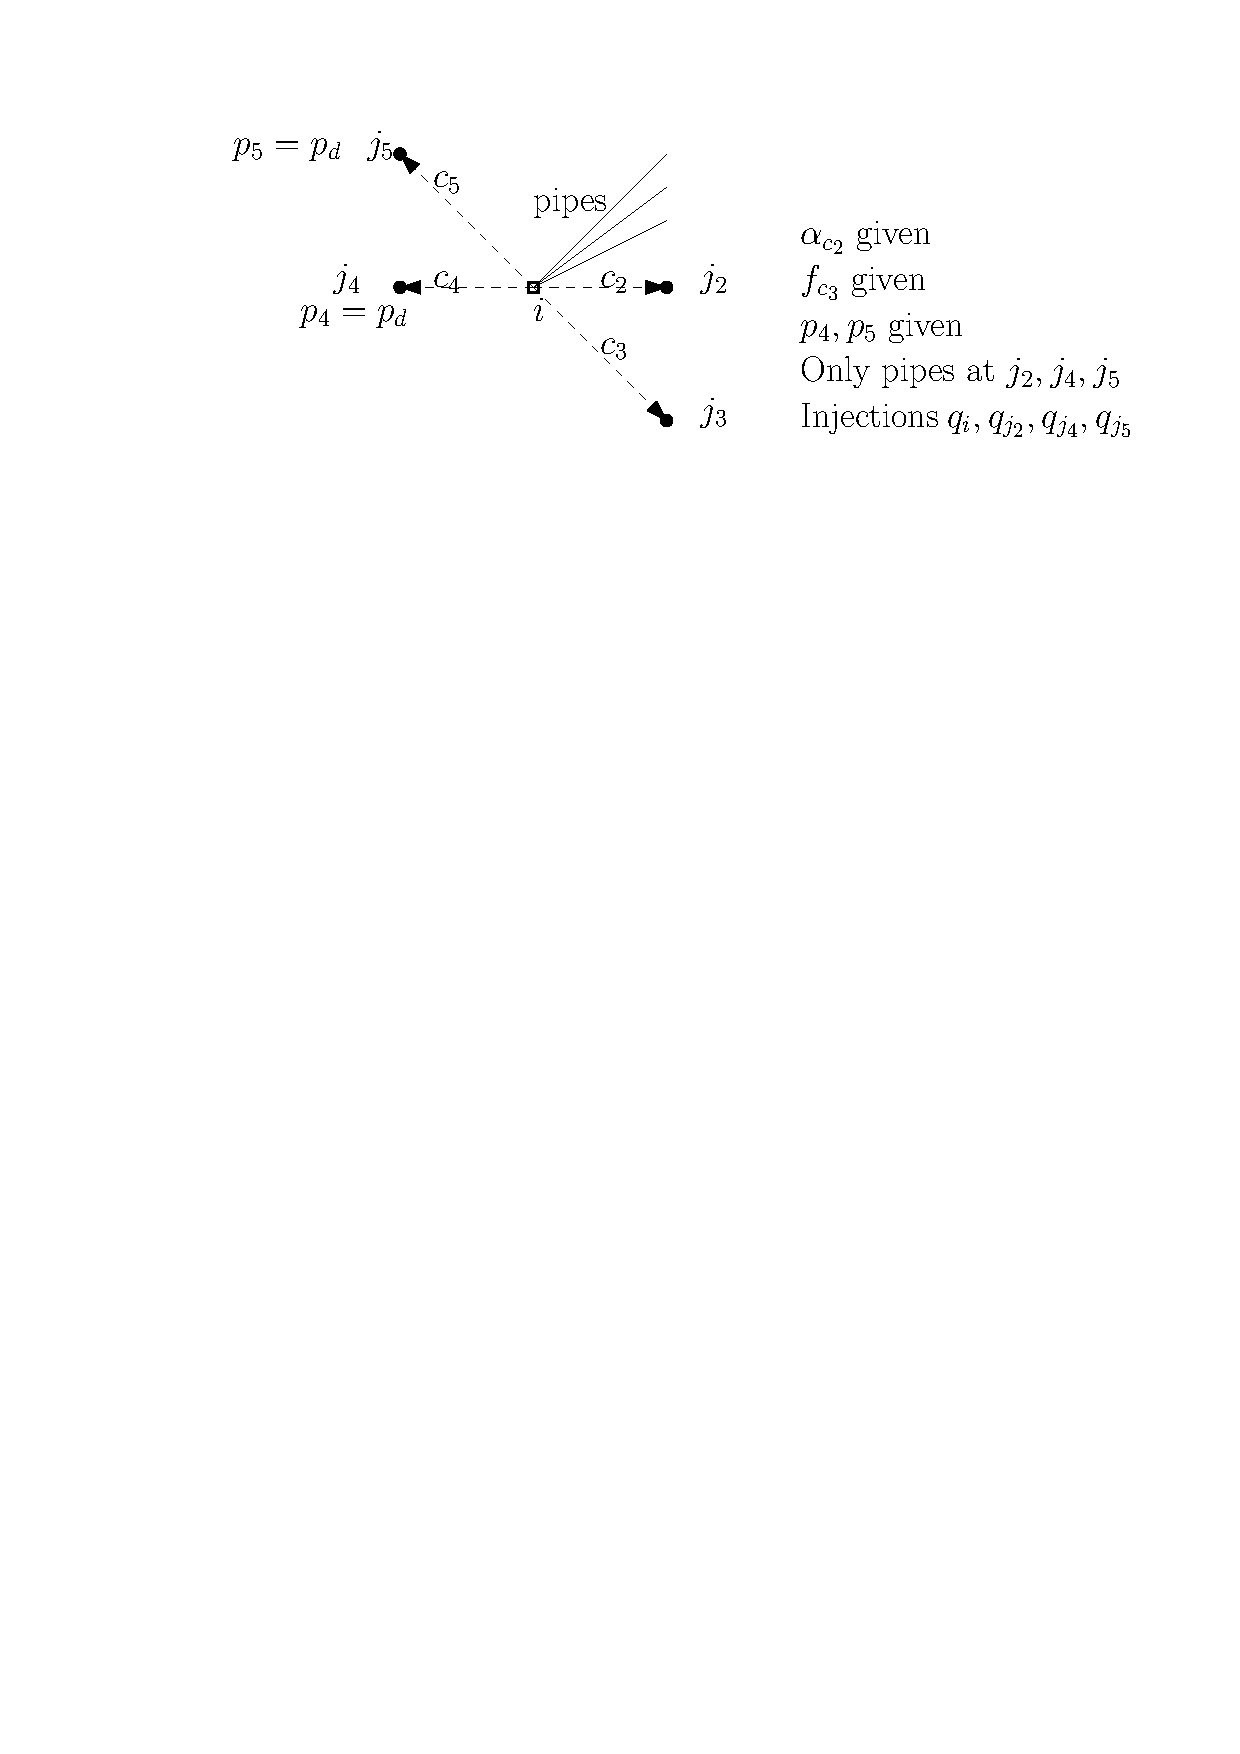
\includegraphics[scale=1]{fig1} \label{fig:config1}}\\
\subfloat[Configuration 2]{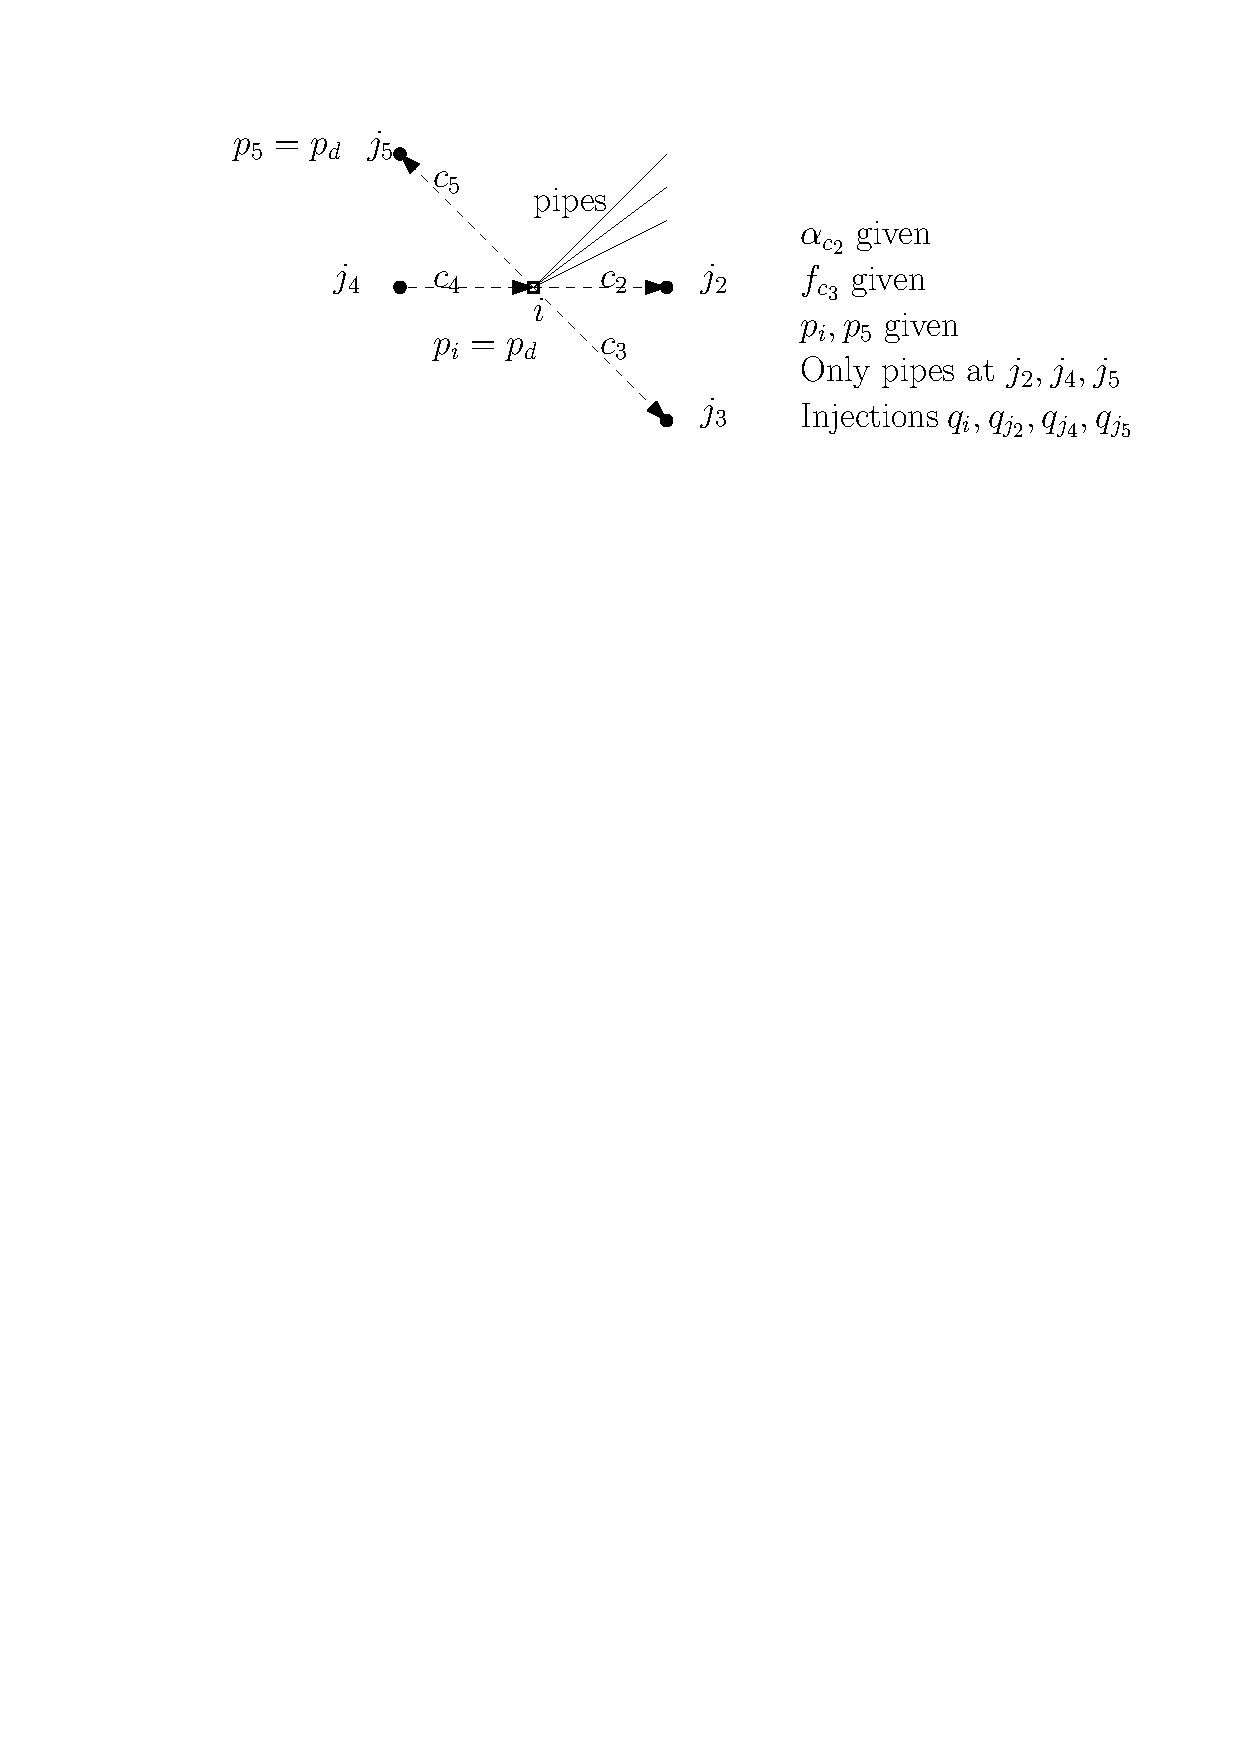
\includegraphics[scale=1]{fig2} \label{fig:config2}}
\caption{Considering vertex $i$, which is a Level 1 vertex, we determine vertex densities at $i$ and its neighbours $j_2, j_3, j_4, j_5$  which are Level 2 vertices connected to $i$ by compressors. The network restrictions stated earlier imply that for these configurations, $c_4$ and $c_5$ can be outgoing compressors, but they cannot both be incoming compressors, and $p_5, p_4$ in Figure~\ref{fig:config1} and $p_5, p_i$ in
Figure~\ref{fig:config2} cannot be slack nodes.}
\label{fig:configs}
\end{figure}



The density at vertex $i$ in the configuration in Figure~\ref{fig:config1} is determined through

\begin{align}
& \left[ \sum_{u \in e(i)}\frac{s_{u} \Delta x_{u}}{\Delta t} + \sum_{u \in e(j_2)}\alpha_{c_2}\frac{s_{u} \Delta x_{u}}{\Delta t} \right] \left( \rho^{n+1}(i) - \rho^n(i) \right) =  \sum_{v \in e(j_4)}\left[\frac{s_{v} \Delta x_{v}}{\Delta t}\right] \cdot \left(\rho^{n}(j_4) - \rho^{(n+1)}(j_4) \right) \notag \\
& + \sum_{v \in e(j_5)}\left[\frac{s_{v} \Delta x_{v}}{\Delta t}\right] \cdot \left(\rho^{n}(j_5) - \rho^{(n+1)}(j_5) \right) 
+\sum_{v \in \{j_2, j_4, j_5, i\}} \left( q^{(n+1/2)}_{v}(t) + \sum_{u \in e(v)}\sgn(u) s_{u} \phi_{u-}^{(n+1/2)}(v) \right) + f^{(n+1/2)}_{c_3}
\label{eqn:config1}
\end{align}

Since $\rho^{(n+1)}(j_4), \rho^{(n+1)}(j_5)$ are already known, once $\rho^{(n+1)}(i)$ is determined from \eqref{eqn:config1}, $\rho^{(n+1)}(j_2)$ is also found. 
In this configuration (Figure~\ref{fig:config1}), we \emph{do not} solve for $\rho^{(n+1)}(j_3)$ but it will be determined separately when we land at vertex $j_3$. The treatment of vertex $j_3$ is different because the compressor $c_3$ has mass-flow specified, and thus it is treated similar to the injection $q(i)$  at the vertex $i$. In practice, we will directly solve for $\rho^{(n+1)}(j_3)$ to ensure that all Level 2 neighbours of $i$ are updated. This is necessary because our strategy is built around visiting  Level 0/1 nodes alone, and simply skipping Level 2 nodes.



In this scenario (see Figure~\ref{fig:config2}, the density at the base vertex $i$ is already known, since we have now reversed the direction of compressor $c_4$. However, we develop the equations for density at vertex $j_4$ as 

\begin{align}
& \left[ \sum_{u \in e(j_4)}\frac{s_{u} \Delta x_{u}}{\Delta t} \right] \left ( \rho^{n+1}(j_4) - \rho^{n}(j_4) \right)  = \sum_{v \in e(j_5)}\left[\frac{s_{v} \Delta x_{v}}{\Delta t}\right] \cdot \left(\rho^{n}(j_5) - \rho^{(n+1)}(j_5) \right)  \notag \\
& + \left[ \sum_{u \in e(i)}\frac{s_{u} \Delta x_{u}}{\Delta t} + \sum_{u \in e(j_2)}\alpha_{c_2}\frac{s_{u} \Delta x_{u}}{\Delta t} \right]\left( \rho^n(i) - \rho^{n+1}(i) \right) \notag \\
& +\sum_{v \in \{j_2, j_4, j_5, i\}} \left( q^{(n+1/2)}_{v}(t) + \sum_{u \in e(v)}\sgn(u) s_{u} \phi_{u-}^{(n+1/2)}(v) \right) + f^{(n+1/2)}_{c_3}
\label{eqn:config2}
\end{align}

It can be seen that equations \eqref{eqn:config1} and \eqref{eqn:config2} 
are identical; we have simply transposed terms to reflect the known and unknown terms.

\begin{itemize}
\item The case of multiple incoming/outgoing compressors such as $c_2$ with given compressor ratios is easy to generalize. The compressor ratio will appear as $1/\alpha_c$ for incoming compressors in \eqref{eqn:config1}, \eqref{eqn:config2}. 
\item Similarly multiple compressors with given massflux are handled in the same way as  $c_3$, i.e., the densities are solved for after determining the density at the Level 1 ``root" vertex $i$.
\item Multiple outgoing compressors with discharge pressure control, such as $c_4$, $c_5$ in Figure~\ref{fig:config1} are no problem.
\item However, if $c_4$ be incoming, it must be the sole incoming compressor with discharge pressure control. Else the vertex equations cannot be solved locally (since it violates condition (2) above)
\end{itemize}

\subsection{Advantages of this formulation}
In case of disruptive events, the network topology may change in the following ways:
\begin{enumerate}
\item A compressor may malfunction, leading to it blocking flow completely (in which case one can change its control to be a low value of mass flow)
\item Opening and closing of valves correspond to control values of mass flow changing from one value to another in a specified time interval
\item A compressor with given ratio may instead be operated to  deliver at a given pressure or vice versa
\end{enumerate}
This list is representative, and by no means exhaustive. However, the point to note is that, network changes of this kind are easy to handle, and it is reflected locally in the equations for the vertex associated with the component.

Note that the time marching step for internal nodes associated with mass flux and density are inherently parallel operations and may be performed as such. However, one can go further and check if it is possible to reduce the set of junctions to the  smallest possible set such that each junction and its neighbours are disjoint from the rest thus ensuring that we can perform computations for each of these vertices in parallel too. In the absence of such a decomposition however,  one must visit each junction serially, 
for parallel operations will result in a race condition.

\section{Data structures and sequence of operations for junction equations}
\begin{enumerate}
\item For a pipe between nodes $i, j$, there will be a grid for $\rho, \phi$. Also, a field to access $\phi^-(i), \phi^-(j)$.
\item For each node, a flag to indicate if its pressure value has been updated in this current step.
\item For each node, a list of \emph{all} pipes and compressors attached, a flag to indicate incoming/outgoing, and a compressor ratio (set to 1 if pipe). Note that this might include information about pipes at neighbouring nodes if compressors with unknown fluxes are present.
\item Then visit each Level 0/1 node, check if pressure value update flag is true; if so, exit and go to next node. Else perform computations at node, and update pressure at neighbouring nodes if relevant.
\item Once all nodes updated, reset pressure update flag to false
\item Now update fluxes
\item We can start with a steady-state solution of $\phi, \rho$ as initial conditions, where we will assume that the nodal injections of the steady-state problem are held constant for time interval $[0, \Delta t/2]$
\end{enumerate}

\section{Global formulation}

The way to solve this problem without any restrictions on network topology is to form the full matrix system and solve the system simulataneously.
\begin{enumerate}
\item Proceed as follows to first calculate the numbers of dofs in the problem, given that there are $N$ nodes in total, of which $N_s$ are slack nodes, and there are $n_c$ compressors.
\item The number of nodal pressure dofs would be $N - N_s$. 
\item For each compressor, we create either (i) 2 dofs, $f_c, 1/\alpha_c$ if delivery pressure is specified or (ii) single dof $f_c$ if $\alpha_c$ is specified, or (iii) no dofs if $f_c(t)$ is given.
\item For each of the $N- N_s$ nodes $i_0$, we write the balance equation that involves the nodal pressure $p(i_0)$, and compressor mass fluxes $f_c$ if unknown. 
\item For each compressor for which $f_c$ is unknown, we write an equation. Either $(1/\alpha_c)p(i_0) - p(j) = 0$ if $\alpha_c$ is given. Else if delivery pressure $p_d$ is given, then $(p_d)1/\alpha_c - p(j) = 0$.
\item The dofs thus comprise of $p_i, f_c, 1/\alpha_c$. If all compressors have mass flow given, only $p_i$ to solve for. If all compressors have $\alpha_c$ given, then solve for $p_i, f_c$.
\item Will need to have a node to dof map and vice versa for use in every time step.
\item The system matrix will be sparse, but because $\alpha_c(t)$ and $\Delta t$ may change with every time step, will need to evaluate in each step. RHS depends on previous time step solution, hence obviously needs updating each step.
However, this algorithm does not take advantage of the local nature  of jucntion computations, and will result in the computational overhead  of repeated calculation and assembly of the global matrix if there are topology changes.
\end{enumerate}

\section{Non-dimensionalization}
Let us choose the nominal quantities $p_0, \rho_0, v_0, \phi_0, t_0, l_0,f_0, A_0$ for pressure, density, velocity, mass flux, time, length, mass flow and cross-sectional area respectively.

Then we can rewrite the governing equations in nondimensional variables $\bar{\rho}, \bar{t},\bar{\phi}, \bar{x}, \dotsc$  through the substitutions $\rho = \rho_0 \bar{\rho}, t = t_0\bar{t}, \dotsc$.

Then $$\dfrac{\partial \bar{\rho}}{\partial \bar{t}} + \left( \dfrac{\phi_0t_0}{\rho_0l_0} \right)\dfrac{\partial \bar{\phi}}{\partial \bar{x}} = 0$$
and
$$\dfrac{\partial \bar{\phi}}{\partial \bar{t}} + \left( \dfrac{p_0t_0}{l_0\phi_0} \right)\dfrac{\partial \bar{p}}{\partial \bar{x}} = -\dfrac{\lambda}{2D}\left( \dfrac{\phi_0t_0}{\rho_0} \right) \dfrac{\bar{\phi}|\bar{\phi}|}{\bar{\rho}}$$

We use a \emph{fixed} value for the speed of sound $a$, choose values for $l_0, p_0, \rho_0, v_0$ based on the data, and set $A_0 =1, \phi_0 = \rho_0 v_0, t_0 = l_0/v_0, f_0 = \phi_0 A_0$.

This choice of values reduces the governing equations to 
$$\dfrac{\partial \bar{\rho}}{\partial \bar{t}} + \dfrac{\partial \bar{\phi}}{\partial \bar{x}} = 0$$
$$\dfrac{\partial \bar{\phi}}{\partial \bar{t}} + \dfrac{\mathcal{C}}{\mathcal{M}^2}\dfrac{\partial \bar{p}}{\partial \bar{x}} = -\left( \dfrac{\lambda}{2D/l_0} \right) \dfrac{\bar{\phi}|\bar{\phi}|}{\bar{\rho}}$$

where $\mathcal{C} =  \dfrac{p_0}{\rho_0 a^2}$ and $\mathcal{M} = \dfrac{v_0}{a}$ are the Euler number and Mach number respectively.
Note that in this process, the equation of state has never been considered. Thus, the non-dimensionalisation is valid for both ideal and non-ideal gas. 


The ideal gas equation, $p = \rho R_g T$ transforms to $\bar{\rho} = \mathcal{C} \bar{p}$ since $a = \sqrt{R_gT}$. In non-isothermal problems, we can we can define a nominal temperature $T_0$  and set $a=\sqrt{R_gT_0}$ in that case to get $\bar{\rho} = \dfrac{\mathcal{C}T_0}{T} \bar{p}$.

For a non-ideal gas, assuming the CNGA equation of state we have $p\cdot(b_1 + b_2 p) = \rho R_g T$ which simplifies to the expression $\bar{\rho} = \left ( \bar{b_1} + \bar{b_2}\bar{p} \right ) \bar{p}$, where $\bar{b_1} = \mathcal{C}b_1, \bar{b_2} = \mathcal{C}p_0 b_2$. 

The speed of sound $a$ in a gas  is given by $a^2 = \dfrac{d p}{d \rho}$. For an ideal gas, we get $a^2 = R_g T$, or in nondimensional terms  $\dfrac{d \bar{p}}{d \bar{\rho}} = 1/\mathcal{C} = \bar{a}^2 $.

For a simple CNGA equation, $p\cdot(b_1 + b_2 p) = \rho R_g T$, we can calculate the sound speed from $\dfrac{d \rho}{d p}$ since $\dfrac{d p}{d \rho} \cdot \dfrac{d \rho}{d p} = 1$. Thus  $a_{CNGA}^2 = \dfrac{R_g T}{b_1 + 2b_2 p}$. Since $b_1 > 1, b_2 > 0, p > 0$, $a_{CNGA} < a$.
We can reach the same conclusion from the fact that  $\dfrac{d \bar{p}}{d \bar{\rho}} = \dfrac{1}{\bar{b_1} + 2\bar{b_2}\bar{p}}$ and $\bar{b_1} > \mathcal{C}, \bar{b_2} > 0$.


Let us record the CFL condition and its consequence next. Usually, it would be stated as $\bar{c}\Delta \bar{t}/ \Delta \bar{x} \leq 1$, but to be safe, we consider 
$\bar{c}\Delta \bar{t}/ \Delta \bar{x} \leq k$ for $k= 0.9$.

Note that $\bar{c} = \dfrac{\mathcal{C}}{\mathcal{M}^2} \sqrt{\dfrac{d \bar{p}}{d \bar{\rho}}}$.
The CFL condition for the ideal gas is the strongest and thus it is sufficient to take $\bar{c} = \dfrac{\sqrt{\mathcal{C}}}{\mathcal{M}^2}$. For the particular choice $v_0 = a$, we  get $\mathcal{C} = \mathcal{M} = \bar{c} = 1$.

Thus, for a given value of $\Delta \bar{t}$, $\Delta \bar{x} \geq \bar{c}\Delta \bar{t}/k$. Setting $\Delta \bar{x} = \bar{L}/m$,  $m \leq \dfrac{\bar{L} k}{\bar{c}\Delta \bar{t}}$.


\section{Inclined pipes}
If the inclination of the pipes is taken into account, then gravity could have a component along the pipe, and if this is taken into account, the formulation needs to be modified slightly.
For the given choice of non-dimensional variables, the momentum equation is modified to
$$\dfrac{\partial \bar{\phi}}{\partial \bar{t}} + \dfrac{\mathcal{C}}{\mathcal{M}^2}\dfrac{\partial \bar{p}}{\partial \bar{x}} = -\left( \dfrac{\lambda}{2D/l_0} \right) \dfrac{\bar{\phi}|\bar{\phi}|}{\bar{\rho}} + 
\left ( \dfrac{l_0g_{||}}{v_0^2} \right )\bar{\rho}$$
Given the elevation of the ``from" and``to" ends of a pipe, $g_{||}$ can be calculated as the component of gravity along the assumed flow direction. The resultant nondimensional number $\mathbb{G}_{\mathrm{pipe}} = \dfrac{l_0 g_{||}}{v_0^2}$ thus varies for each pipe, and is not a constant for the network.

\end{document}